\chapter{1D Positional experiments - 3 Categories} \label{Chapter: 1DPosition}

\newlength\figureheight
\newlength\figurewidth


\section{Experimental setup}
EDIT IMAGES
Crowdflower \footnote{ http://crowdflower.com/} is an online service that allows for simple tasks to be posted to a number of crowdsourcing worker markets. By providing a wrapper and common API for several crowdsourcing provides, Crowdflower boasts the largest crowd of workers out of any platform. Due to limitations in its API, only relatively simple tasks can be posted. Crowdflower was used to post a series of simple images to the crowd, getting feedback from hundreds of workers.

All the following experiments consisted of showing a static image of a circle to workers who were required to pick the best 1 of 2 or more avaiable options which described the location of the circle in the image. 

Each worker was shown a series of images, where the position of the circle changed from image to image, with each worker providing a single response for each image. A total of 11 images were shown to each worker, with the position of the circle ranging from 0 to 1 \footnote{The units are arbitrary, but the values $0:0.1:1$ are used throughout}, as shown in \ref{Figure:1d_position_images} . For each experiment, a simple html page was created with the images stored in a public Dropbox folder. 


% 1d circle pictures
\begin{figure}
  \centering
  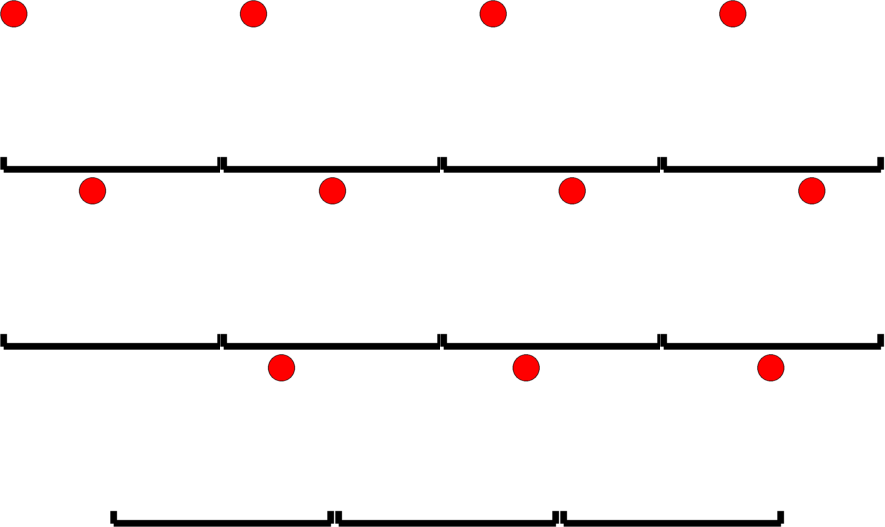
\includegraphics[width=8cm]{combined_1d_images.png}
  \caption{The images posted to the crowd. These show the circle at positions $0:0.1:1$ giving a total of 11 images }
  \label{Figure:1d_position_images}
\end{figure}

\section{3 Category Decisions}
Let \possResVec be an \nPossRes valued discrete variable that represents the possible worker responses, where $\possResVec \in \mathbb{N}$ .Workers were asked to describe the position of the circle using one of three responses $\realPossResVec = \lbrace 'NearTheLeft', 'NearTheCentre' , 'NearTheRight'\rbrace$, which were mapped to $\possResVec=\lbrace 1,2,3 \rbrace$, setting $\nPossRes=3$.An example of the worker GUI is shown in \ref{Figure:crowdflower_question_3} (current screenshot does not show image as dropbox is not accessible from BAE systems - get another screenshot). Each worker was shown a total of  11 images. 

%%worker GUI png
\begin{figure}
  \centering
  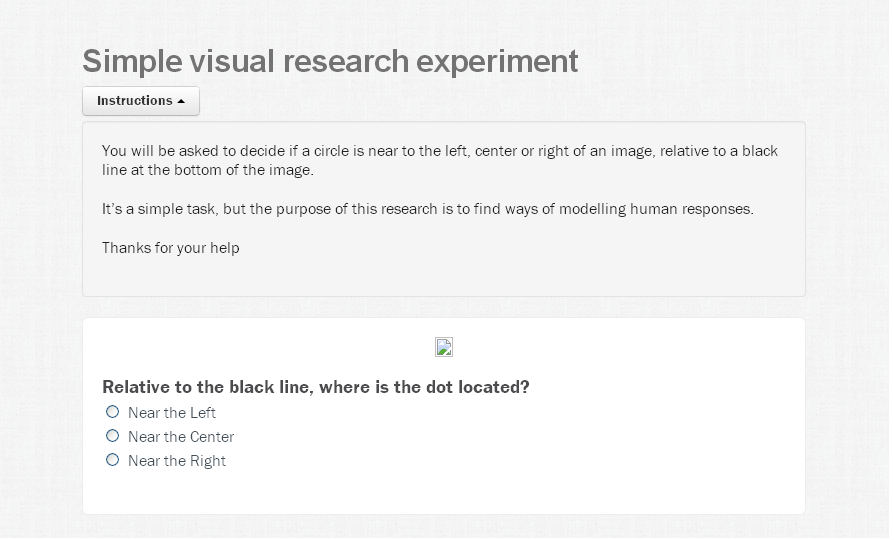
\includegraphics[width=8cm]{crowdflower_gui_noimage.png}
  \caption{The task window for a worker, requiring one of three responses}
  \label{Figure:crowdflower_question_3}
\end{figure}

A total of 100 workers were asked to provide feedback, leading to a dataset of 1100 responses. 1 worker set, for some reason, was provided by two workers (with one worker providing 10 responses, and another 1 response), so the total number of usable workers was 99

The aim is to estimate the ground truth position of the circle given a response from 1 or more workers. 

\subsection{Dataset}

A large amount of data is returned by crowdflower, including worker responses, their declared location, their IP address, the crowdsourcing platfrom that they provided responses through, and the time each response was received. \tref{Table:text responses} shows a sample of three columns of the returned data which will be useful for the following analysis.


% raw table responses
\begin{table}
\centering
    \begin{tabular}{|l|l|l|}
    \hline
    \textbf{worker id} &    \textbf{image description} & \textbf{responses}       \\ \hline
    16800977      & dot located at 0.3   & Near the Left   \\
    17519077      & dot located at 0.0   & Near the Left   \\
    2666559       & dot located at 0.7   & Near the Right  \\
    16800977      & dot located at 0.5   & Near the Centre \\
    16362086      & dot located at 0.4   & Near the Centre \\ \hline
    \end{tabular}
    \caption{Example of relevant data collected}
  \label{Table:text responses}
\end{table}


In order to make analysis simpler, the strings of data in \tref{Table:text responses} were transformed in to numerical data as shown in \tref{Table:ordinal responses}.


\begin{table}
\centering
    \begin{tabular}{|l|l|l|}
    \hline
    \textbf{workers}  & \textbf{ground truth} & \textbf{responses} \\ \hline
    16800977 & 0.3          & 1         \\
    17519077 & 0.0          & 1         \\
    2666559  & 0.7          & 3         \\
    16800977 & 0.5          & 2         \\
    16362086 & 0.4          & 2         \\ \hline
    \end{tabular}
    \caption{Translation of text responses in to numerical ordinal responses }
  \label{Table:ordinal responses}
\end{table}





Let the random state variable $\possCirclePos \in \mathbb{R}$ be the circles true position. For this experiment the circle can take on one of $\nPossCirclePos=11$ possible positions given by $\possCirclePos = \lbrace 0.0,0.1,...,0.9,1.0 \rbrace$. Each worker $\workIndex$ provides a single response for each circle location. We can define the set of responses for a single worker as the vector $\workResVec_\workIndex$ where each element $\workResVec_{\workIndex,\gtIndex} \in \possResVec$, and $\workResVec_{\workIndex,\gtIndex}$ is the response of worker $\workIndex$ for true circle position $\possCirclePos_\gtIndex$



\section{Initial Analysis}

We can visualise the responses from workers as a bar chart as shown in \ref{Figure:bar responses no gold}. This chart shows the number of left, centre and right responses from all the workers at each of the true circle positions. From this chart we can see that the majority of the responses appear to be reasonable.

%Convert to PNG!
%\begin{figure}
%	\centering
%	\def\svgwidth{10cm}
%	\small
%	\import{../Figures/bar_all_responses/}{bar_all_responses.pdf_tex}
%	\caption{The number of 'NearToLeft', 'NearToRight' and 'NearToCentre' %responses at each position of the circle.}
%	\label{Figure:bar responses no gold}
%\end{figure}





\subsection{Individual Worker Response Models}

Each worker provides a single response at each true circle position. We can create a \textit{ response model} for each worker which simply describes that workers response at each position. A model for an individual is given by the workers response vector $\workResVec_\workIndex$. An example of a response model is shown in \ref{Figure:one worker model}

%convert to png!
%\begin{figure}
%	\centering
%	\def\svgwidth{10cm}
%	\small
%	\import{../Figures/line_single_response_curve/}%{line_single_response_curve.pdf_tex}
%	\caption{Response model for a single worker}
%	\label{Figure:one worker model}
%\end{figure}

\subsubsection{Unique Response Model Groups}
Workers can be grouped by their respective models. Each group is formed by workers who have identical response models i.e. at every true circle position $\possCirclePos_\gtIndex$, they reported the same position category. By grouping workers together, we are able to see the number of different response models there are. The top three most common response models are shown in \ref{Figure:top worker response models}. There was found to be 24 unique response model groups, 10 of which had more than 1 worker with that model, as shown in \ref{Figure:bar unique response model groups}

%\begin{figure}
%	\centering
%	\def\svgwidth{10cm}
%	\small
%	\import{../Figures/line_top_5_response_curves/}{line_top_5_response_curves.pdf_tex}
%	\caption{The top 5 unique response models}
%	\label{Figure:top worker response models}
%\end{figure}

%\begin{figure}
%	\centering
%	\def\svgwidth{10cm}
%	\small
%	\import{../Figures/bar_number_of_workers_per_group/}{bar_number_of_workers_per_group.pdf_tex}
%	\caption{The number of workers in each unique response model group}
%	\label{Figure:bar unique response model groups}
%\end{figure}

\subsubsection{Model Consistency}
We can define a response model as consistent if the difference between adjacent values in a workers response vector are always $\geqslant 0$, or $\leqslant 0$. We can define the response change, the change between adjacent values in a workers response vector $\workResVec_\workIndex$, as
\[\resChange=\workResVec_{\workIndex,\gtIndexCons+1}-\workResVec_{\workIndex,\gtIndexCons}\]
where $\gtIndexCons=\lbrace 1,2,...,\nPossCirclePos -1 \rbrace $

We can define three types of consistent model 

\[
\modType=
\begin{cases}
\consInc & \text{if } \forall \gtIndex, \resChange \geq 0 \text{ and } >0 \text{ for some \workIndex} \\
\consDec      & \text{if } \forall \gtIndex, \resChange \leq 0 \text{ and } < 0 \text{ for some \workIndex}\\
\consCon    & \text{if } \forall \gtIndex, \resChange = 0 
 \end{cases}
\]

where \consInc are increasing models, \consDec are decreasing models and \consCon are constant models. We expect the majority of consistent models to be increasing models, as the true position of the circle increases from left to right for each element of $\workResVec_\workIndex$. A constant consistent model represents a worker who supplied the same response no matter what the circles position. This points towards a worker who either did not understand the question, or more likely did not attempt the question at all - they simply filled in the submission form as quickly as possible. A consistent decreasing model would imply a user who either did not understand the question, or someone who is intentionally providing poor responses.\ref{Figure:increasing worker models} shows all the increasing response models. The number of workers with each increasing response model is shown in \ref{Figure:bar increasing models}

%\begin{figure}
%	\centering
%	\begin{subfigure}{7cm}
%	\def\svgwidth{7cm}
%	\small
%	\import{../Figures/line_all_consistent_increasing/}%{line_all_consistent_increasing.pdf_tex}
%	\caption{}
%	\label{Figure:increasing worker models}
%	\end{subfigure}
%	\begin{subfigure}{7cm}
%	\def\svgwidth{7cm}
%	\small
%	\import{../Figures/bar_consistent_increasing/}{bar_consistent_increasing.pdf_tex}
%	\caption{}
%	\label{Figure:bar increasing models}
%	\end{subfigure}
%	\caption{Increasing consistent response models \subref{Figure:increasing worker models}) All the unique models with increasing response consistency \subref{Figure:bar increasing models}) The number of workers with each increasing model }
%\end{figure}





\subsubsection{Model Symmetry}
Some of the models showed \textit{symmetry},(Is it symmetry? How do we define it?). Let $f_{s}(\workResVec)$
be a function which transforms a workers response vector, so that each 1 is transformed to 3, and a 3 is transformed to 1. Two types of symmetry can be defined


\[
\modType=
\begin{cases}

\resSym & \text{if } \forall \gtIndex, f_{s}(\workResVec_{\workIndex,\gtIndex})=\workResVec_{\workIndex,(\nPossCirclePos+1-\gtIndex)} \text{ and }\workResVec_{\workIndex,\gtIndex}\neq\workResVec_{\workIndex,(\nPossCirclePos+1-\gtIndex)} \text{ for some } \gtIndex  \\

\trueSym      & \text{if } \forall \gtIndex, \workResVec_{\workIndex,\gtIndex}=\workResVec_{\workIndex,(\nPossCirclePos+1-\gtIndex)}\\ 
 \end{cases}
\]

where \resSym is response symmetry, and \trueSym is true symmetry. A model has true symmetry if, at locations $0.5 + a$ and $0.5 - a$ the worker gives the same response. This is an undesirable type of model, as it means that using only this type of model, we would be unable to distinguish between positions such as 0.4 and 0.6.

Response symmetry is where at locations $0.5 + a$ and $0.5-a$, a worker gives the \textit{opposite} response. For example, if they responded 'NearTheRight' at $0.3$, they would responded 'NearTheLeft' at position $0.7$. A response symmetric model looks the same when rotated through $180^\circ$. A worker who responds only 'NearTheCentre' for every true position of the circle is defined to have a model type \trueSym. \ref{Figure:symmetry models} shows the symmetric models.The majority of symmetric models are of the type \resSym

%\begin{figure}
%	\centering
%	\begin{subfigure}{7cm}
%	\def\svgwidth{7cm}
%	\small
%	\import{../Figures/line_true_symmetric_models/}{line_true_symmetric_models.pdf_tex}
%	\caption{}
%	\label{Figure:true symmetric models}
%	\end{subfigure}
%	\begin{subfigure}{7cm}
%	\def\svgwidth{7cm}
%	\small
%	\import{../Figures/line_response_symmetric_models/}{line_response_symmetric_models.pdf_tex}
%	\caption{}
%	\label{Figure:response symmetric models}
%	\end{subfigure}
%	\caption{Symmetric models \subref{Figure:true symmetric models}) True symmetric models \subref{Figure:response symmetric models}) Response symmetric models }
%\end{figure}


\subsection{Time Analysis}

Other than the responses of each worker, the start and finish time of each worker was available. This data only tells us when each worker began the task, and when she finished it - it does not tell us the amount of time they spent on each response.

FIGURE shows the average response time for each worker. The average response time is simply given by 

\[ 
\text{Average response time} = \frac{\text{Total task time}}{\text{Number of responses}}
\]

\begin{figure}
\centering
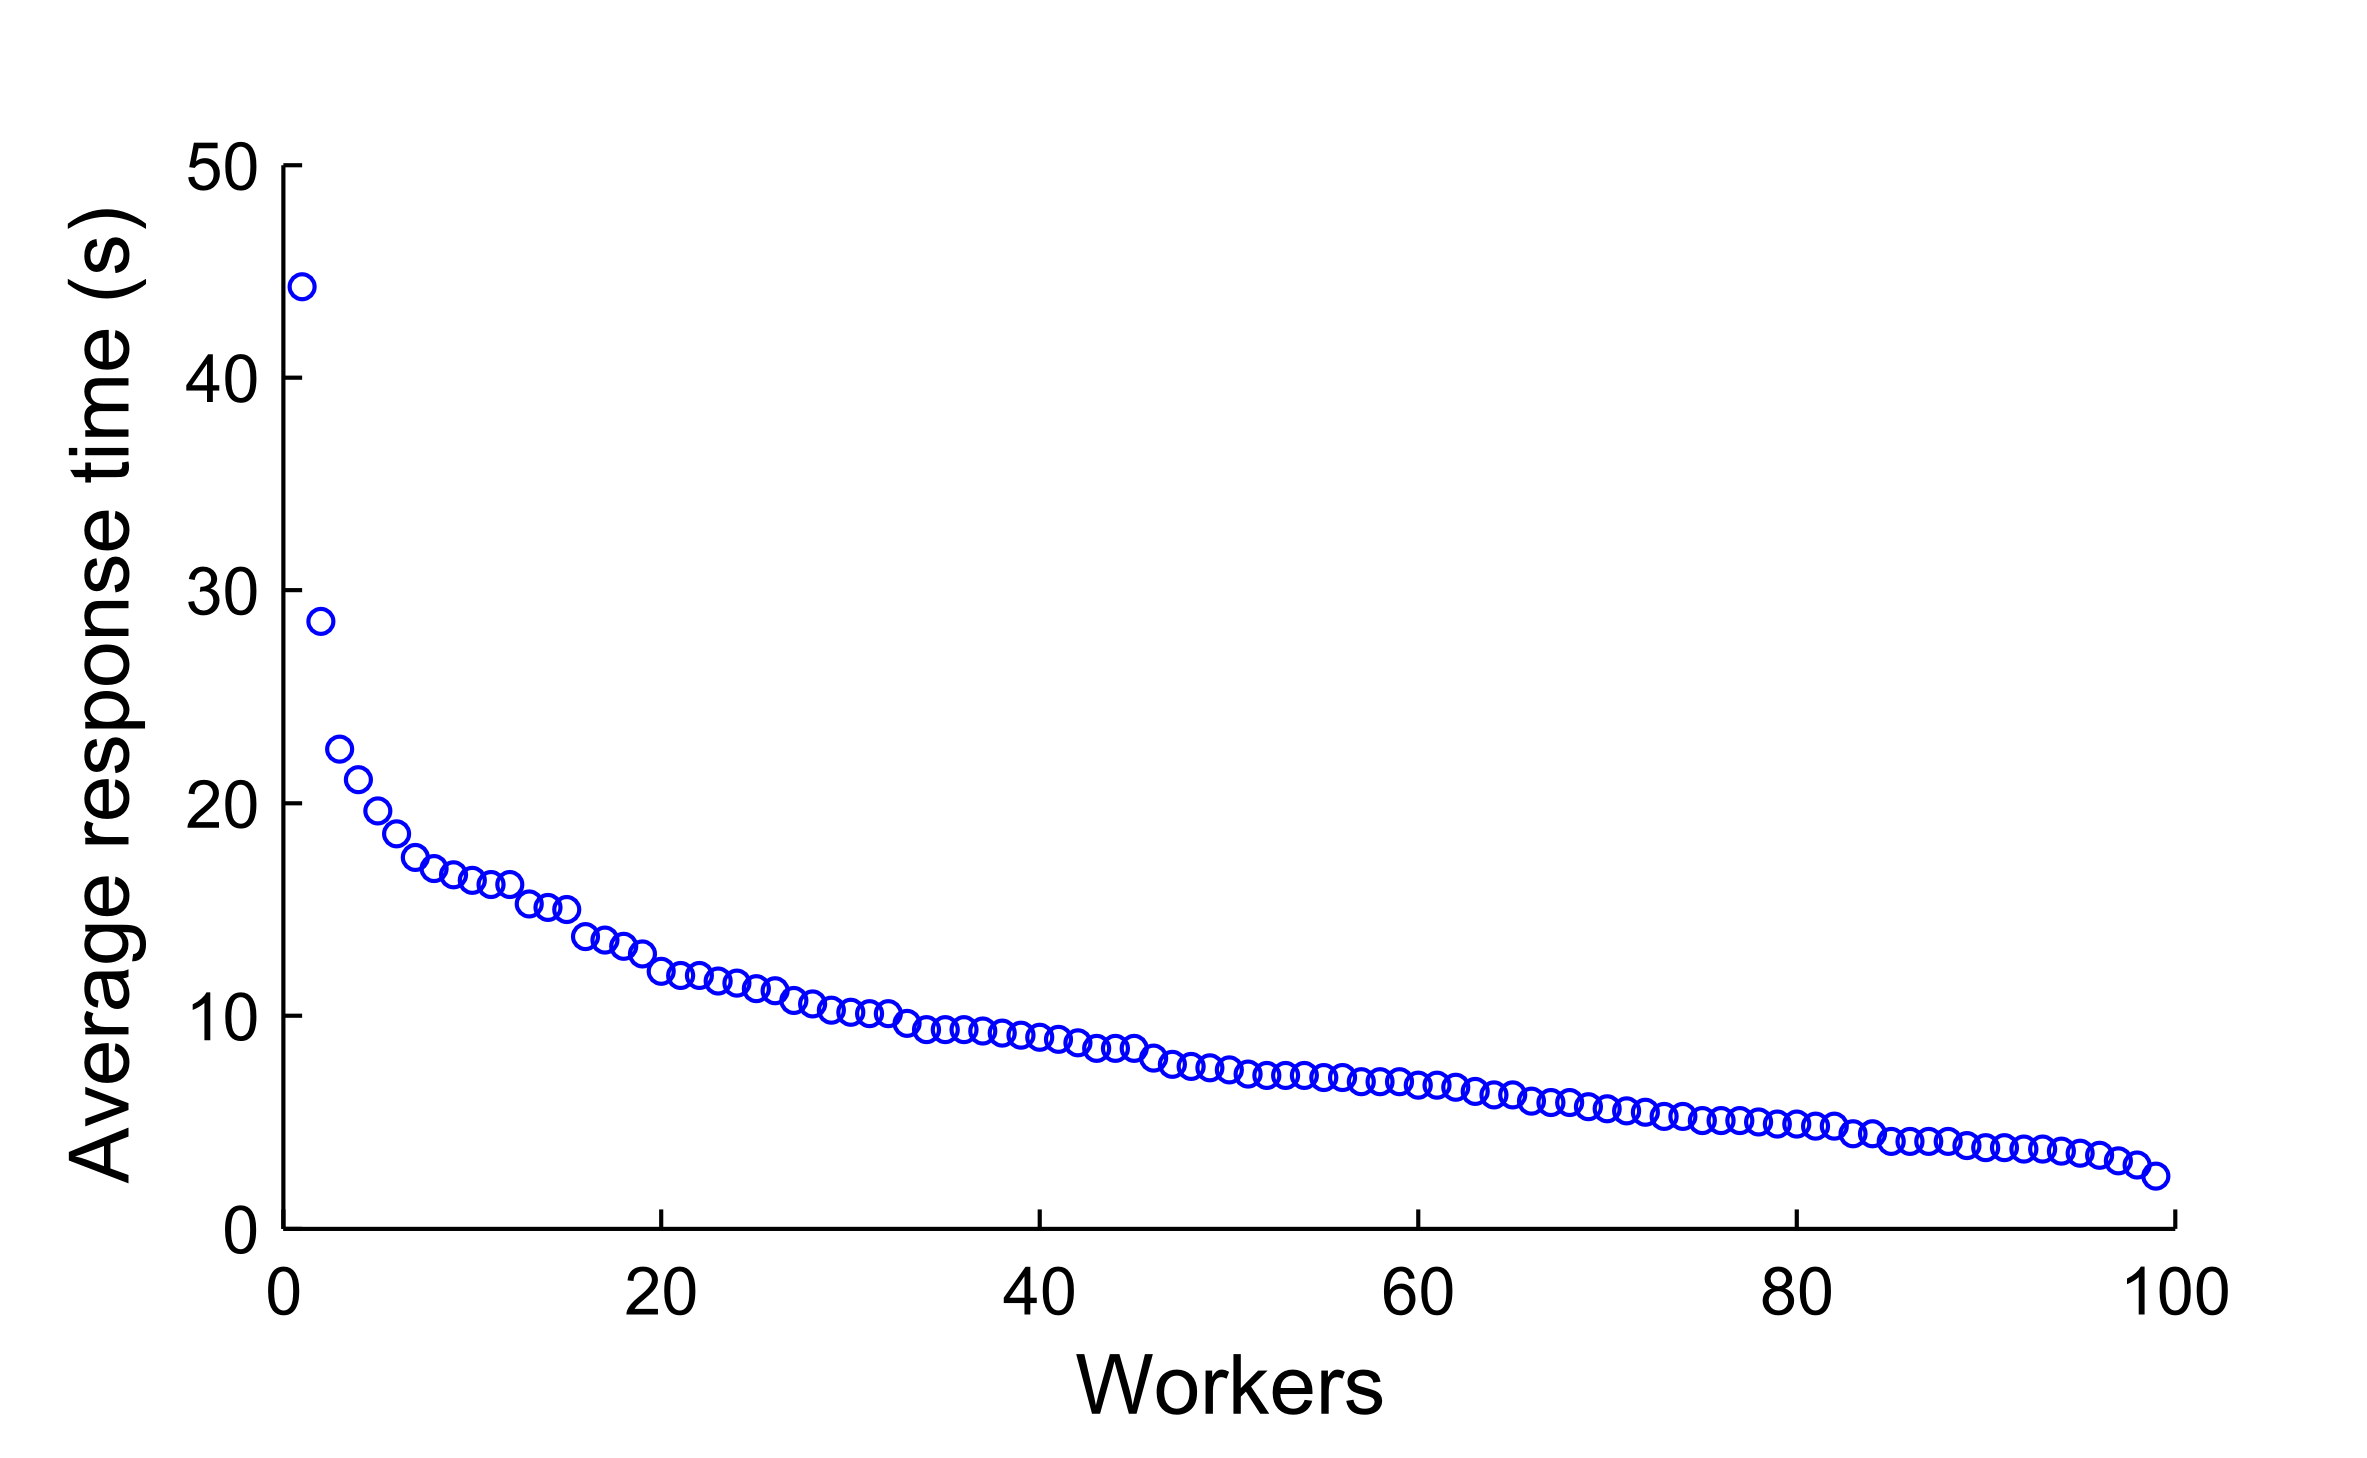
\includegraphics[width=10cm]{line_time_all_responses.png}
\caption{The ranked average response time for each worker.  }
\label{Figure: average_response_time}
\end{figure}



\section{Softmax model fitting}



\section{Initial Fusion Results}

%\begin{figure}
%	\centering
%		\begin{subfigure}{0.5\textwidth}
%			\centering
%			\setlength\figurewidth{10cm}
%    		\setlength\figureheight{5cm}  
%    		\inputTikZ{0.5}{responses_1-99_find0.5_train_on_all.fig.tikz}
%        	\subcaption{}\label{Subfigure:posterior responses raw 0.5}
%        \end{subfigure}%
%       	\begin{subfigure}{0.5\textwidth}
%			\centering
%			\setlength\figurewidth{10cm}
%    		\setlength\figureheight{5cm}  
%    		\inputTikZ{0.5}{responses_1-99_find0.7_train_on_all.fig.tikz}
%        	\subcaption{}\label{Subfigure:posterior responses raw 0.7}
%        \end{subfigure}%
%    	\\
%    	\begin{subfigure}{0.5\textwidth}
%			\centering
%			\setlength\figurewidth{10cm}
%    		\setlength\figureheight{5cm}  
%    		\inputTikZ{0.5}{responses_1-99_find0.4_train_on_all.fig.tikz}
%        	\subcaption{}\label{Subfigure:posterior responses raw 0.4}
%        \end{subfigure}%
%        \begin{subfigure}{0.5\textwidth}
%			\centering
%			\setlength\figurewidth{10cm}
%    		\setlength\figureheight{5cm}  
%    		\inputTikZ{0.5}{responses_1-99_find0.1_train_on_all.fig.tikz}
%        	\subcaption{}\label{Subfigure:posterior responses raw 0.1}
%        \end{subfigure}%
%        \caption{Examples of posterior estimate of circles position with increasing number of responses. Here the softmax model has been trained on all the available data}
%        \label{Figure: posterior responses raw}
%\end{figure}



FIGURE shows the typical impact on the posterior distribution as reports arrive, in the case of unfiltered data, with all of the dataset having been used to train the softmax model. In general the posterior becomes more peaked as more reports arrive. We can see in FIGURE that the distribution tends towards the true value as more reports arrive. In FIGURE we can see that as we increase the number of reports, the estimate becomes more stable. In FIGURE, we see an example of the reports leading to a poor estimate of circle position. In this case, there is a bias in the model that leads to the mean to be over estimated.  





The main process used for this analysis was to train the softmax model using approximately 50\% of the data, and then test the performance using the remaining data. This is repeated through several simulated runs, where the training data is randomly sampled from the full dataset. 


First, lets look at one typical simulation run. In this example, the circle is placed at the value 0.7. As we receive responses from workers, we can update our estimate of where the circle is. \ref{Figure:fusion_find_07} shows the impact of reports coming in on the mean and variance of the posterior distribution. Initially, we receive a report of 'NearTheLeft' which in this case leads to an inital poor estimate of the circles position. The next three reports all state 'NearTheRight' which has the effect of shifting the posterior mean towards the right and leading to an improved estimate of circle position. The complete posterior distribution is shown in \ref{Figure:fusion_find_07_dists}, which shows the reduction in variance as more reports arrive. 

\begin{figure}
	\centering
	\begin{subfigure}{6.5cm}
	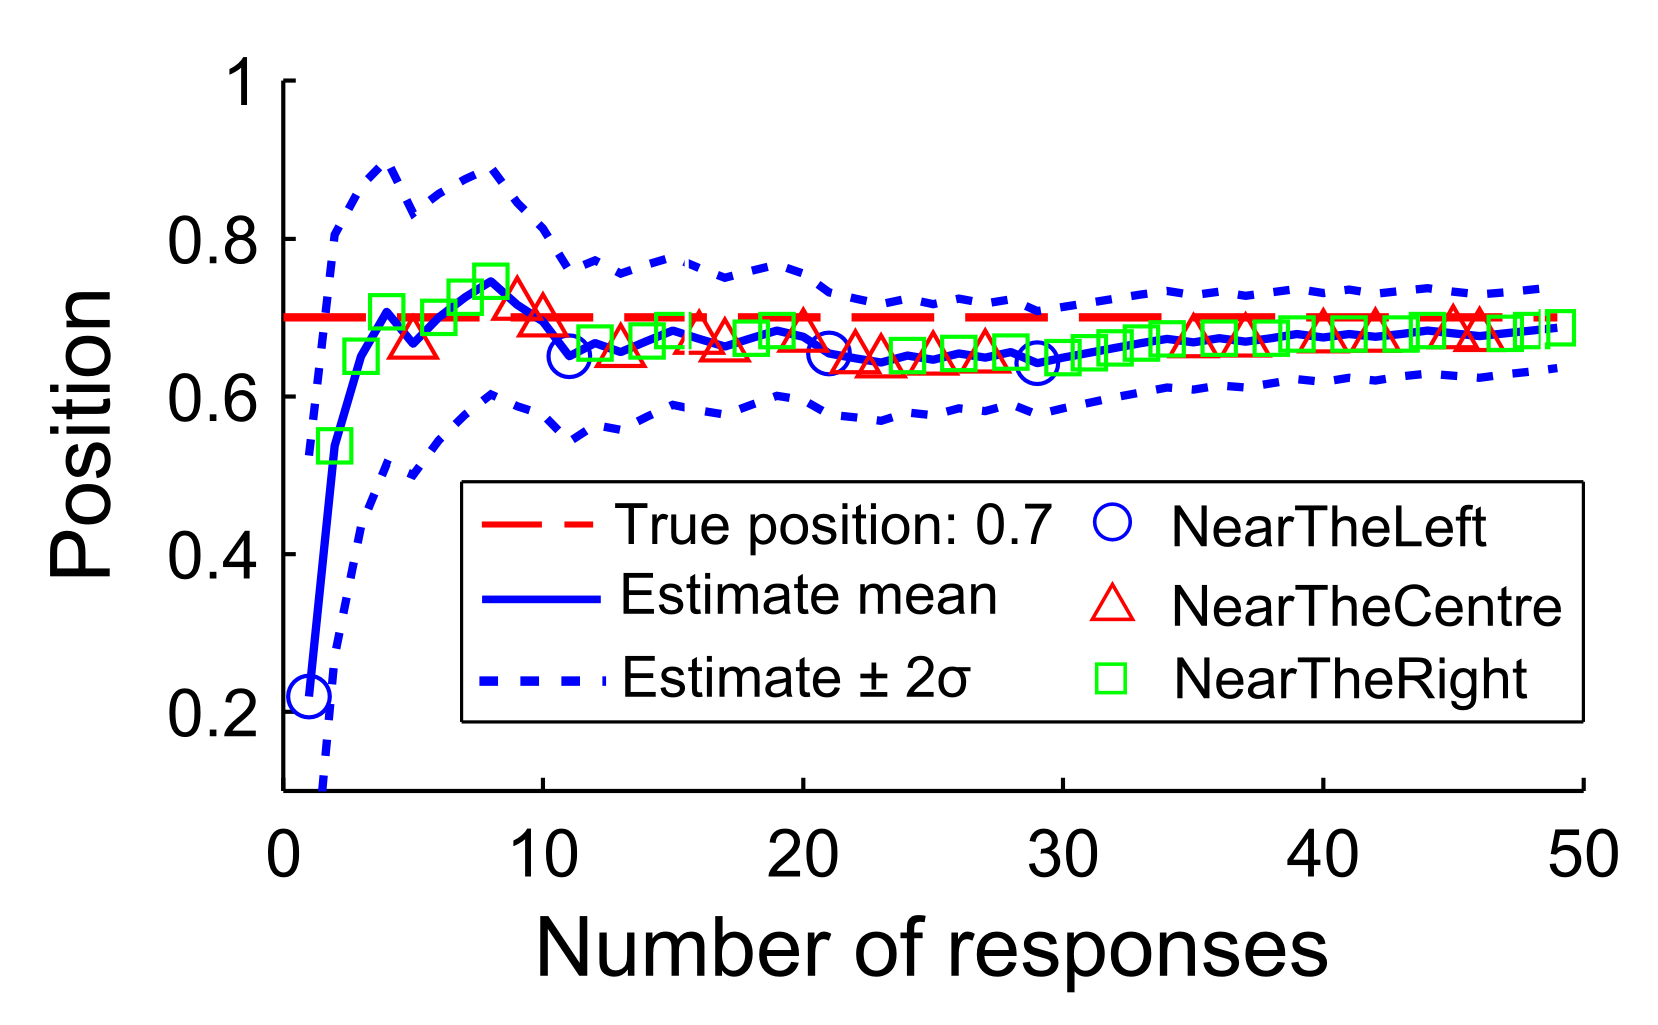
\includegraphics[width=6.5cm]{line_find_07.png}
	\caption{}
	\label{Figure:fusion_find_07}
	\end{subfigure}
	\begin{subfigure}{6.5cm}
	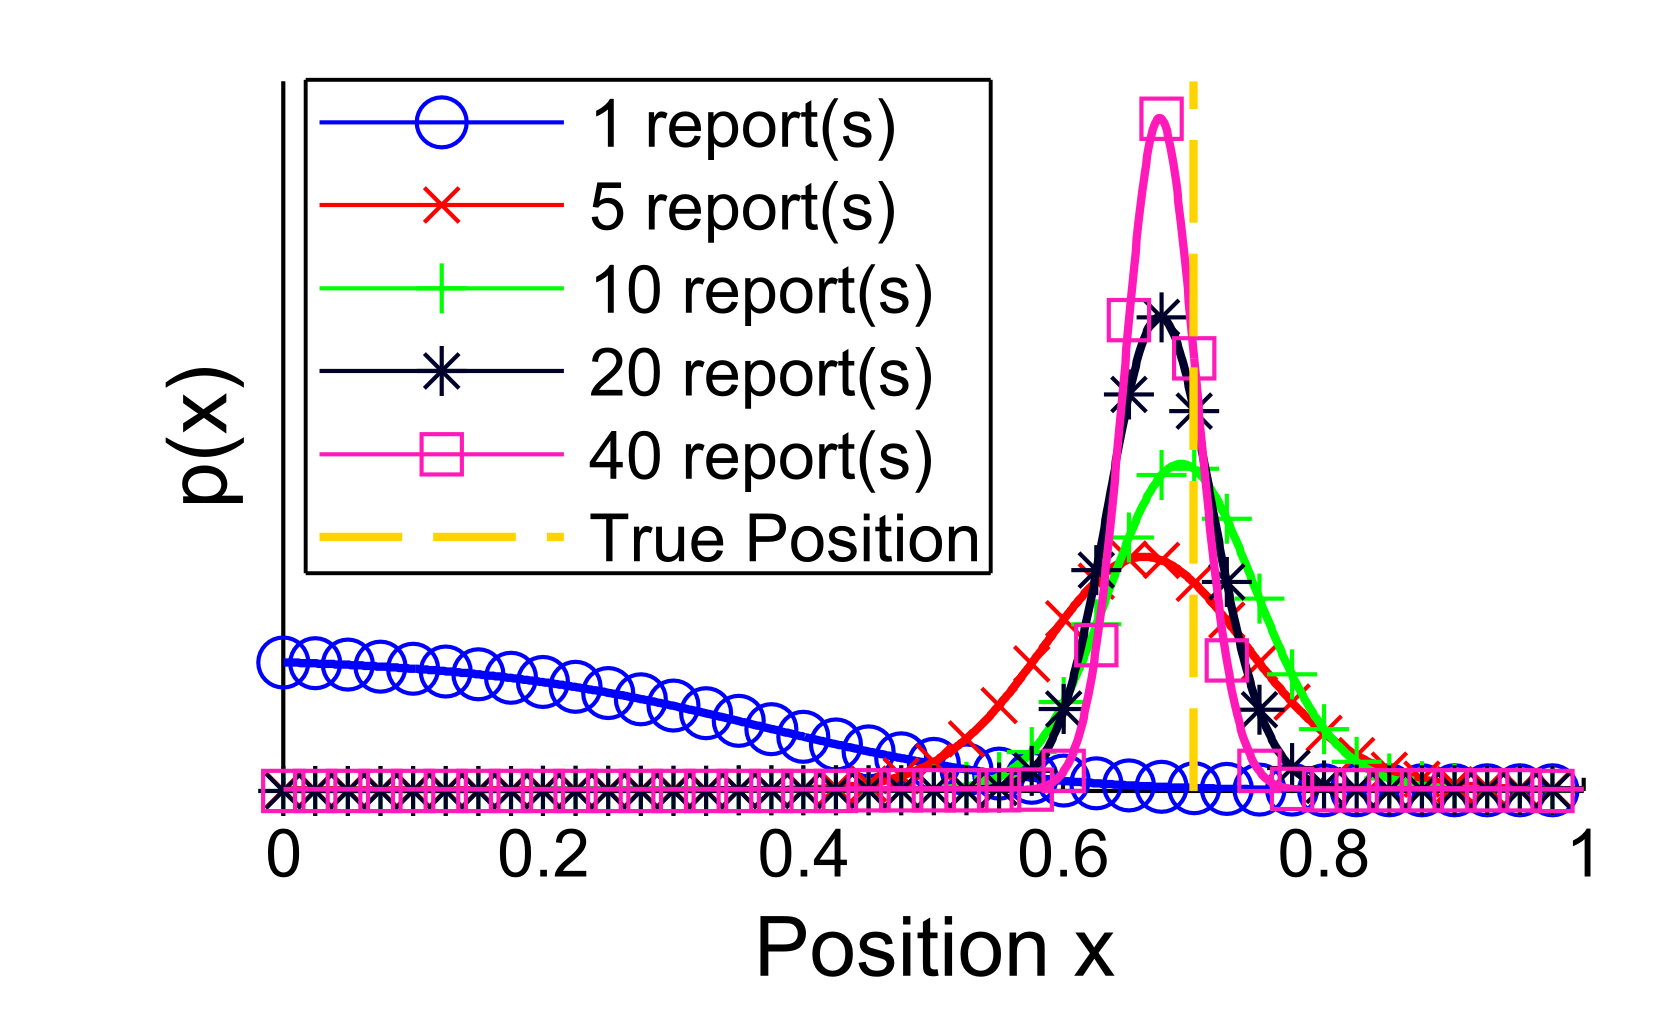
\includegraphics[width=6.5cm]{line_find_07_dists.png}
	\caption{}
	\label{Figure:fusion_find_07_dists}
	\end{subfigure}
	\caption{Estimating the position of the circle as new reports are received  \subref{Figure:fusion_find_07}) The change in posterior mean and variance with responses \subref{Figure:fusion_find_07_dists}) Examples of posterior distribution}
\end{figure}

\ref{Figure:MC RMSE} shows the RMSE for each circle position over 50 simulation runs, as the number of responses is increased. The RMSE was measured between the mean of the posterior distribution and the true circle position. The worst performance is achieved at the outer points 0.0 and 1.0. This can be attributed to the performance metric of the mean, or expectation value, of the distribution being used. At the outer regions of the experiment, the posterior distribution becomes heavily skewed, making the mean a poor summary statistic in this case. It is difficult to summarise multimodal or skewed distributions using a single metric.

The best performing position is 0.5. Again, this is to be expected as the mean of the 'NearTheCentre' likelihood function is close to 0.5, so if the majority of reports are of this type, we would expect a posterior with mean close to 0.5 even after only a small number of reports.


\begin{figure}
	\centering
	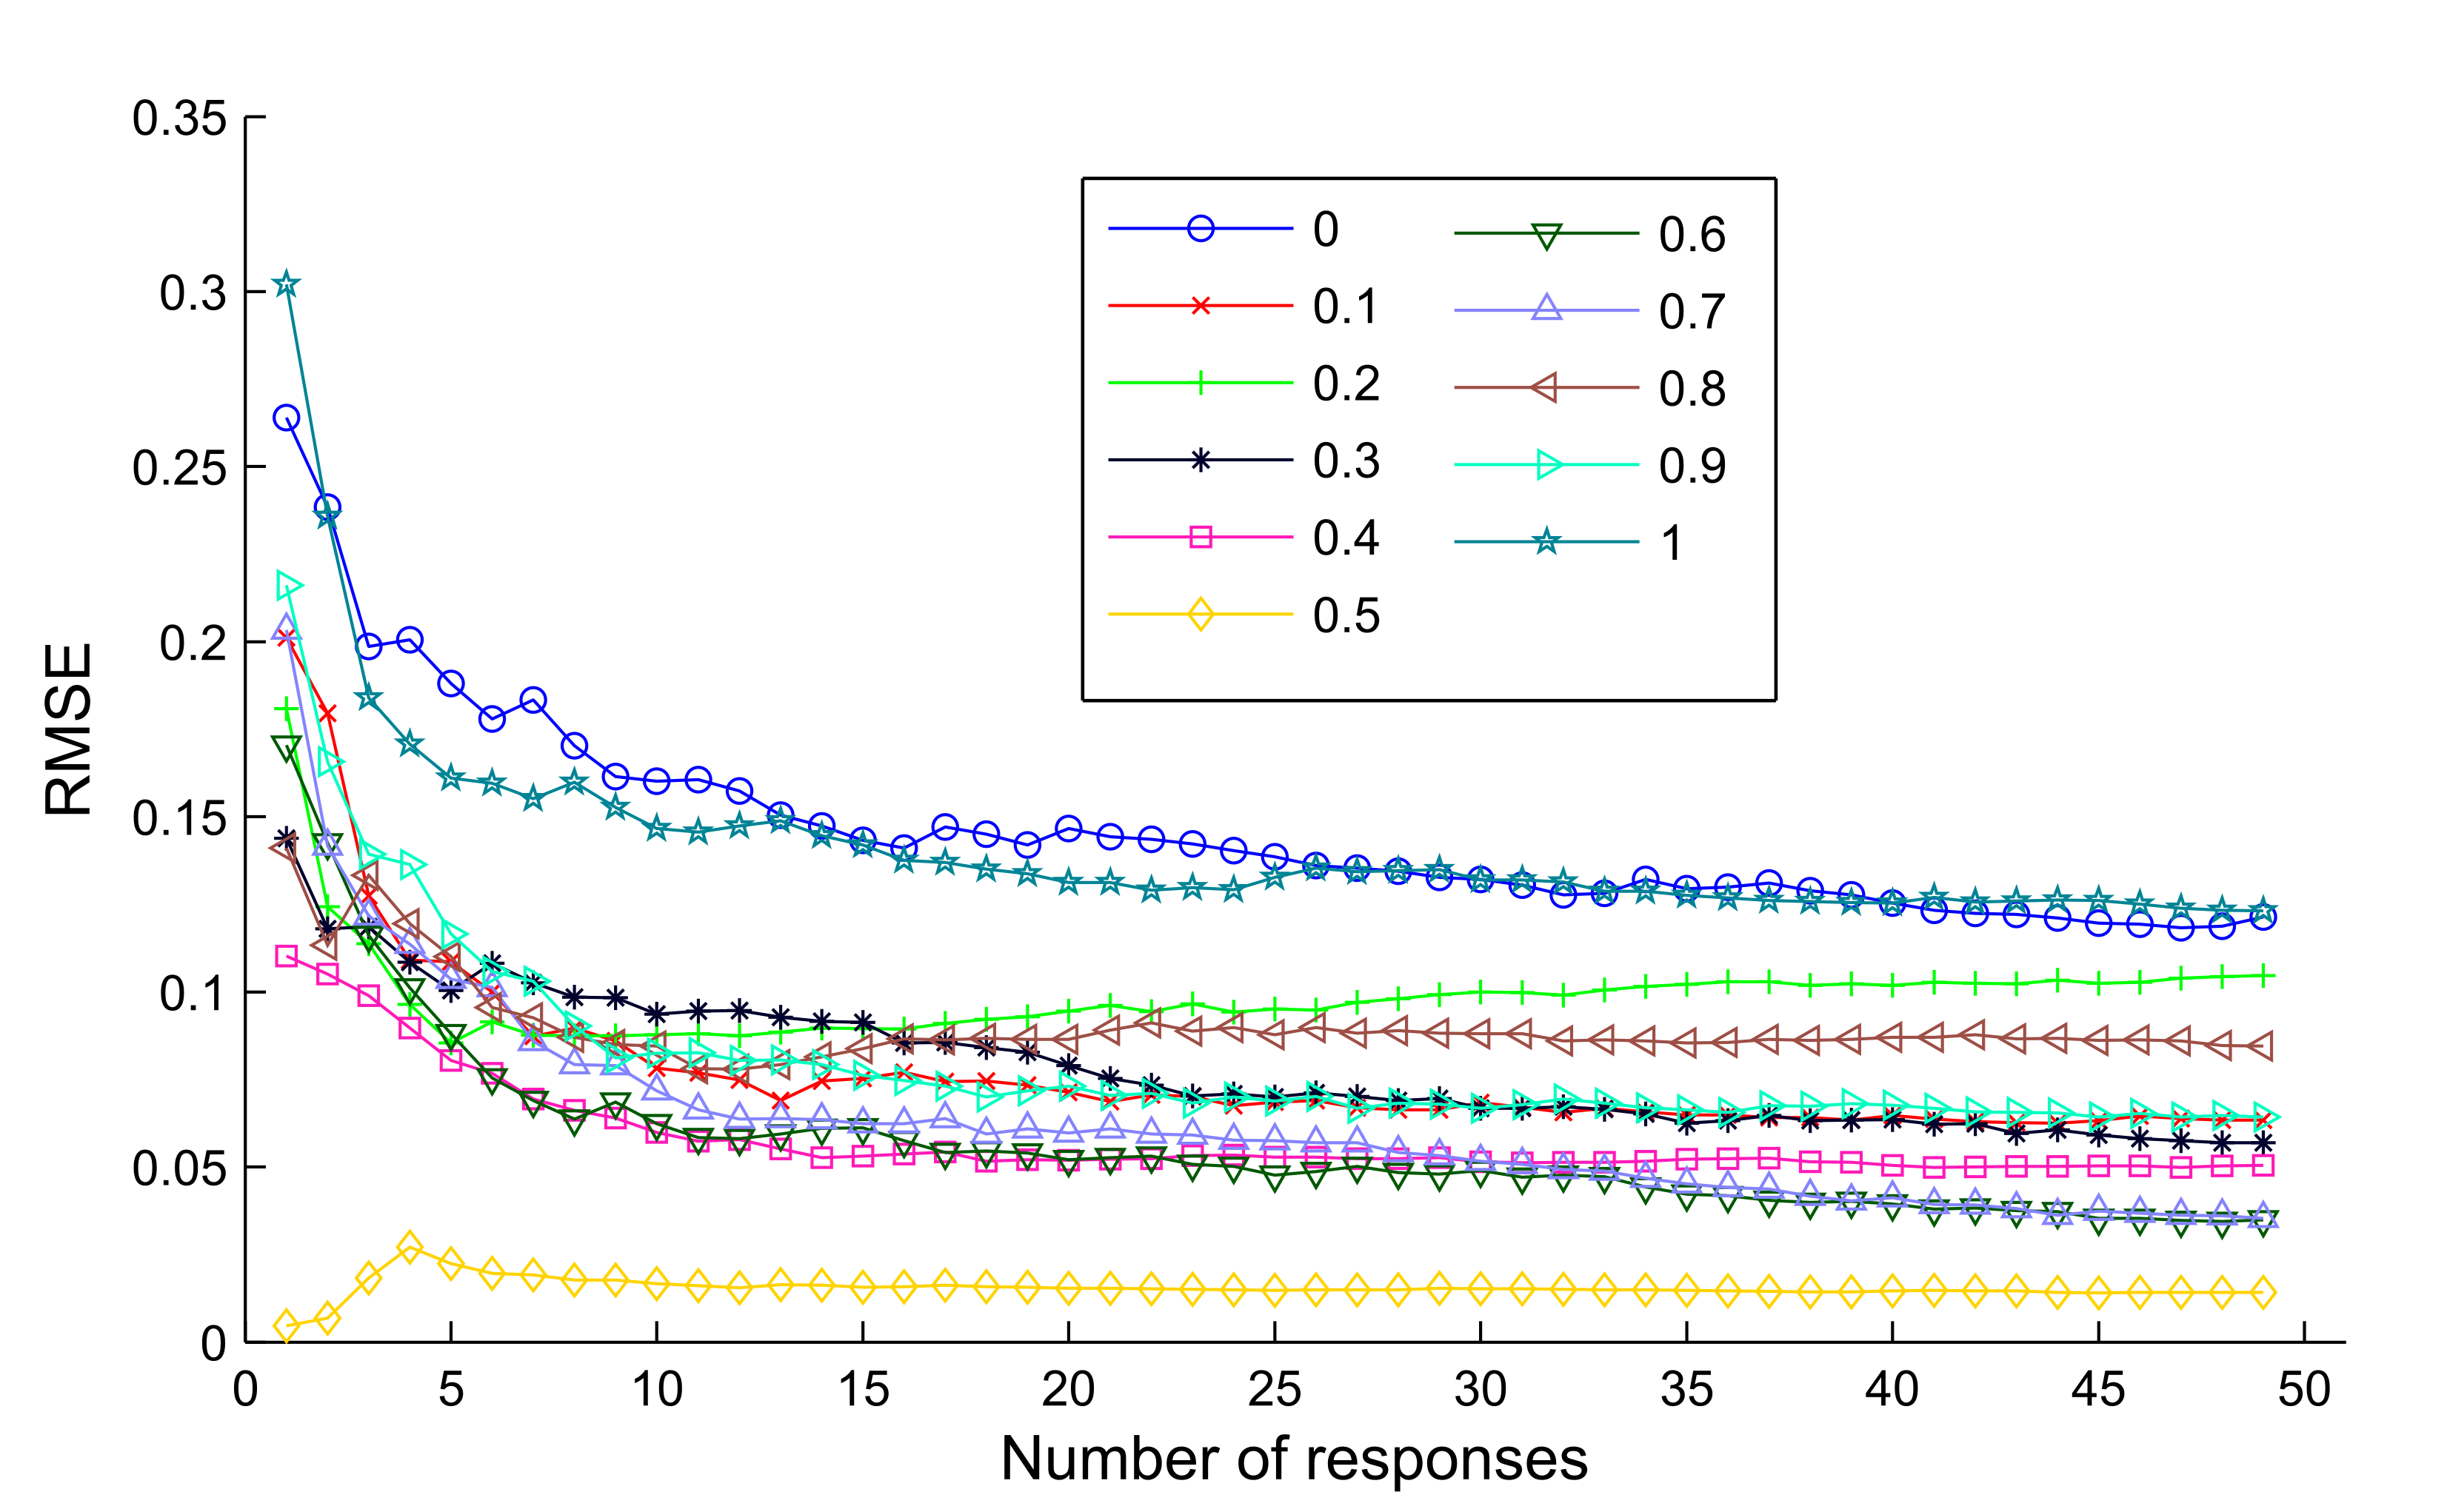
\includegraphics[scale=1]{line_RMSE.png}
	\label{Figure:MC RMSE}
	\caption{The Root-Mean-Square-Error of the posterior with the circle at varying positions, as the number of responses is increased. The RMSE was generated over 50 simulation runs}
\end{figure}


We can view the performance of the fusion by viewing the true circle position against the predicted circle position. This is shown in \ref{Figure: response_estimate}

\begin{figure}
\centering
\begin{subfigure}{6cm}
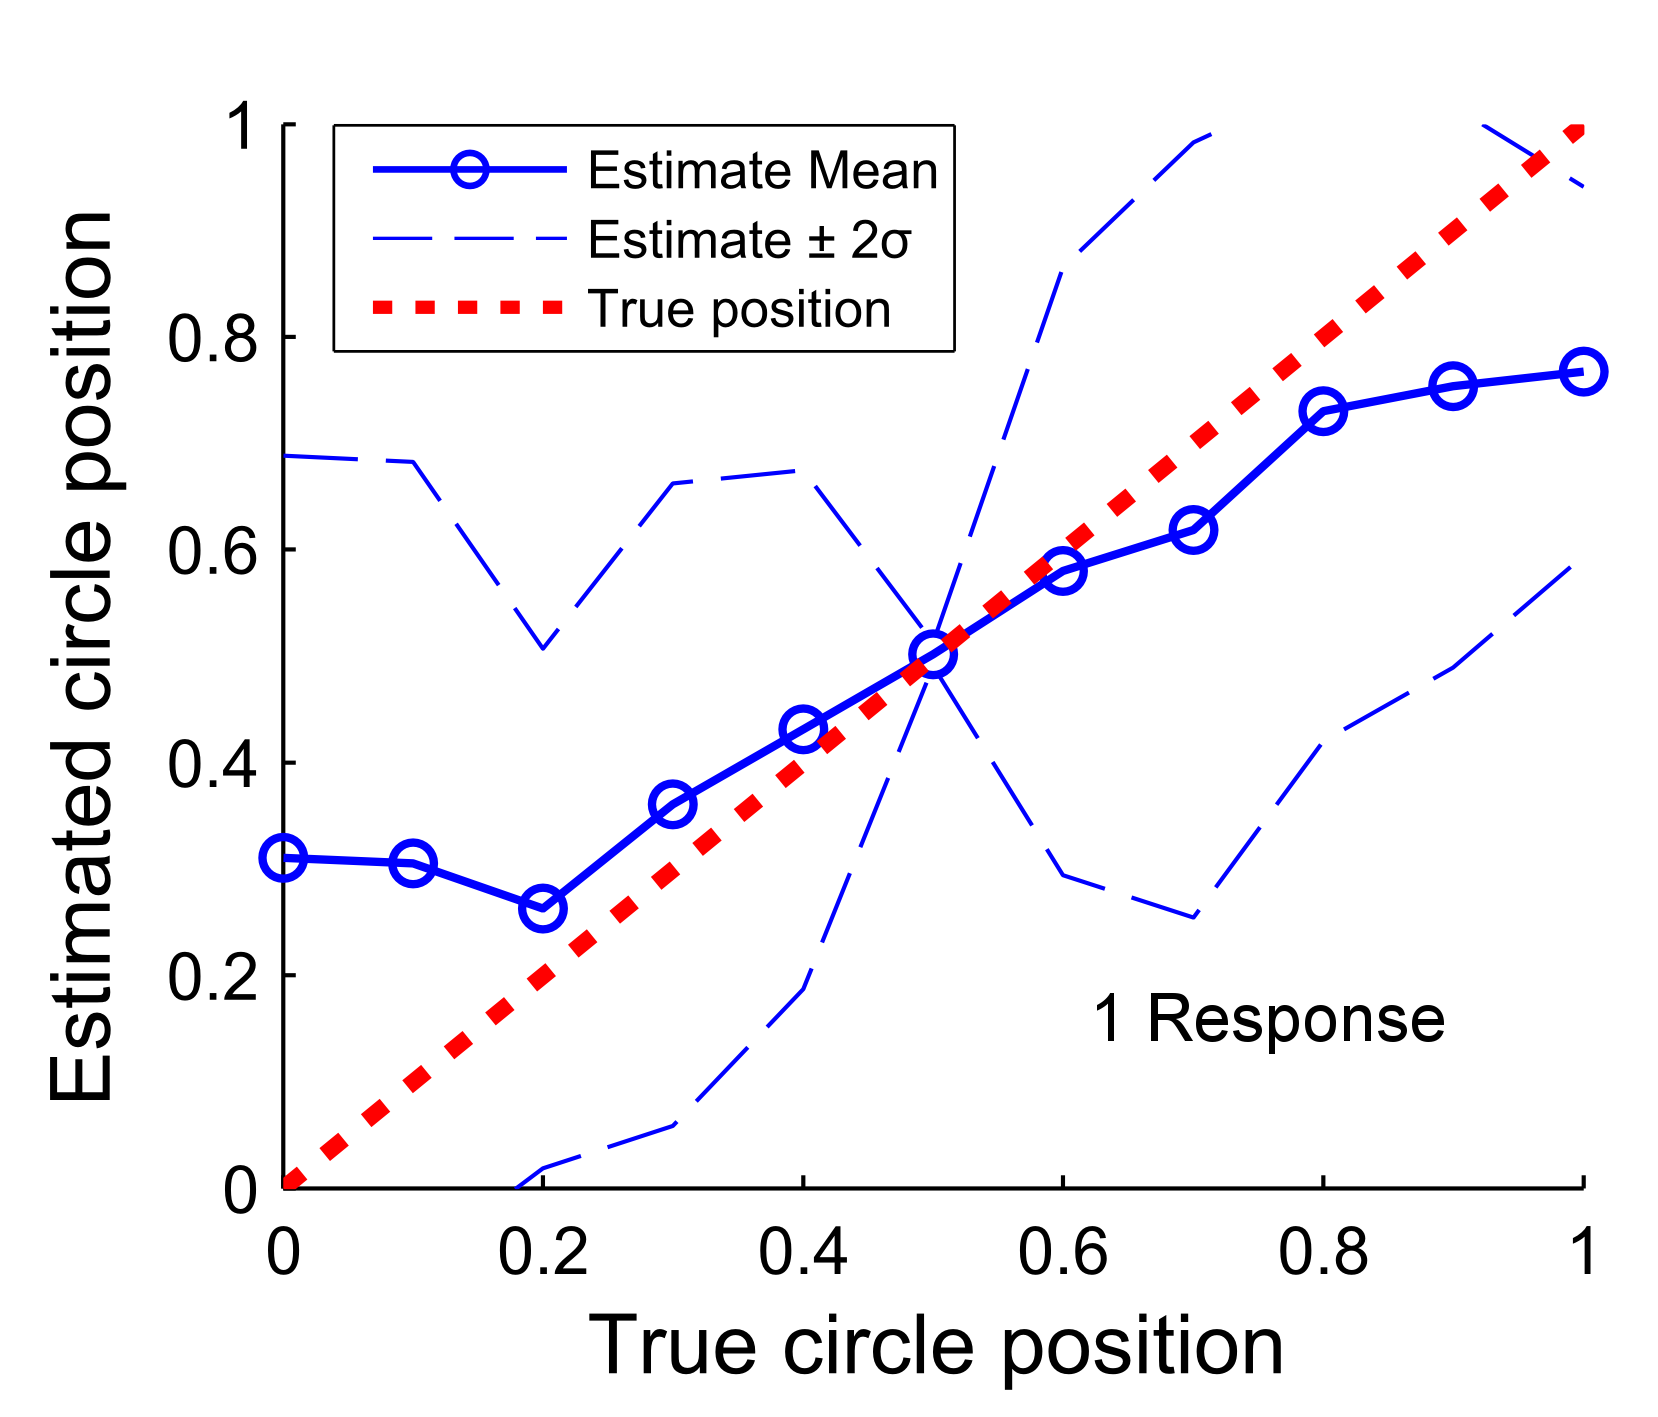
\includegraphics[width=6cm]{line_mc_1res_estimate.png}
\caption{}
\label{Figure: response_estimate_1}
\end{subfigure}
\begin{subfigure}{6cm}
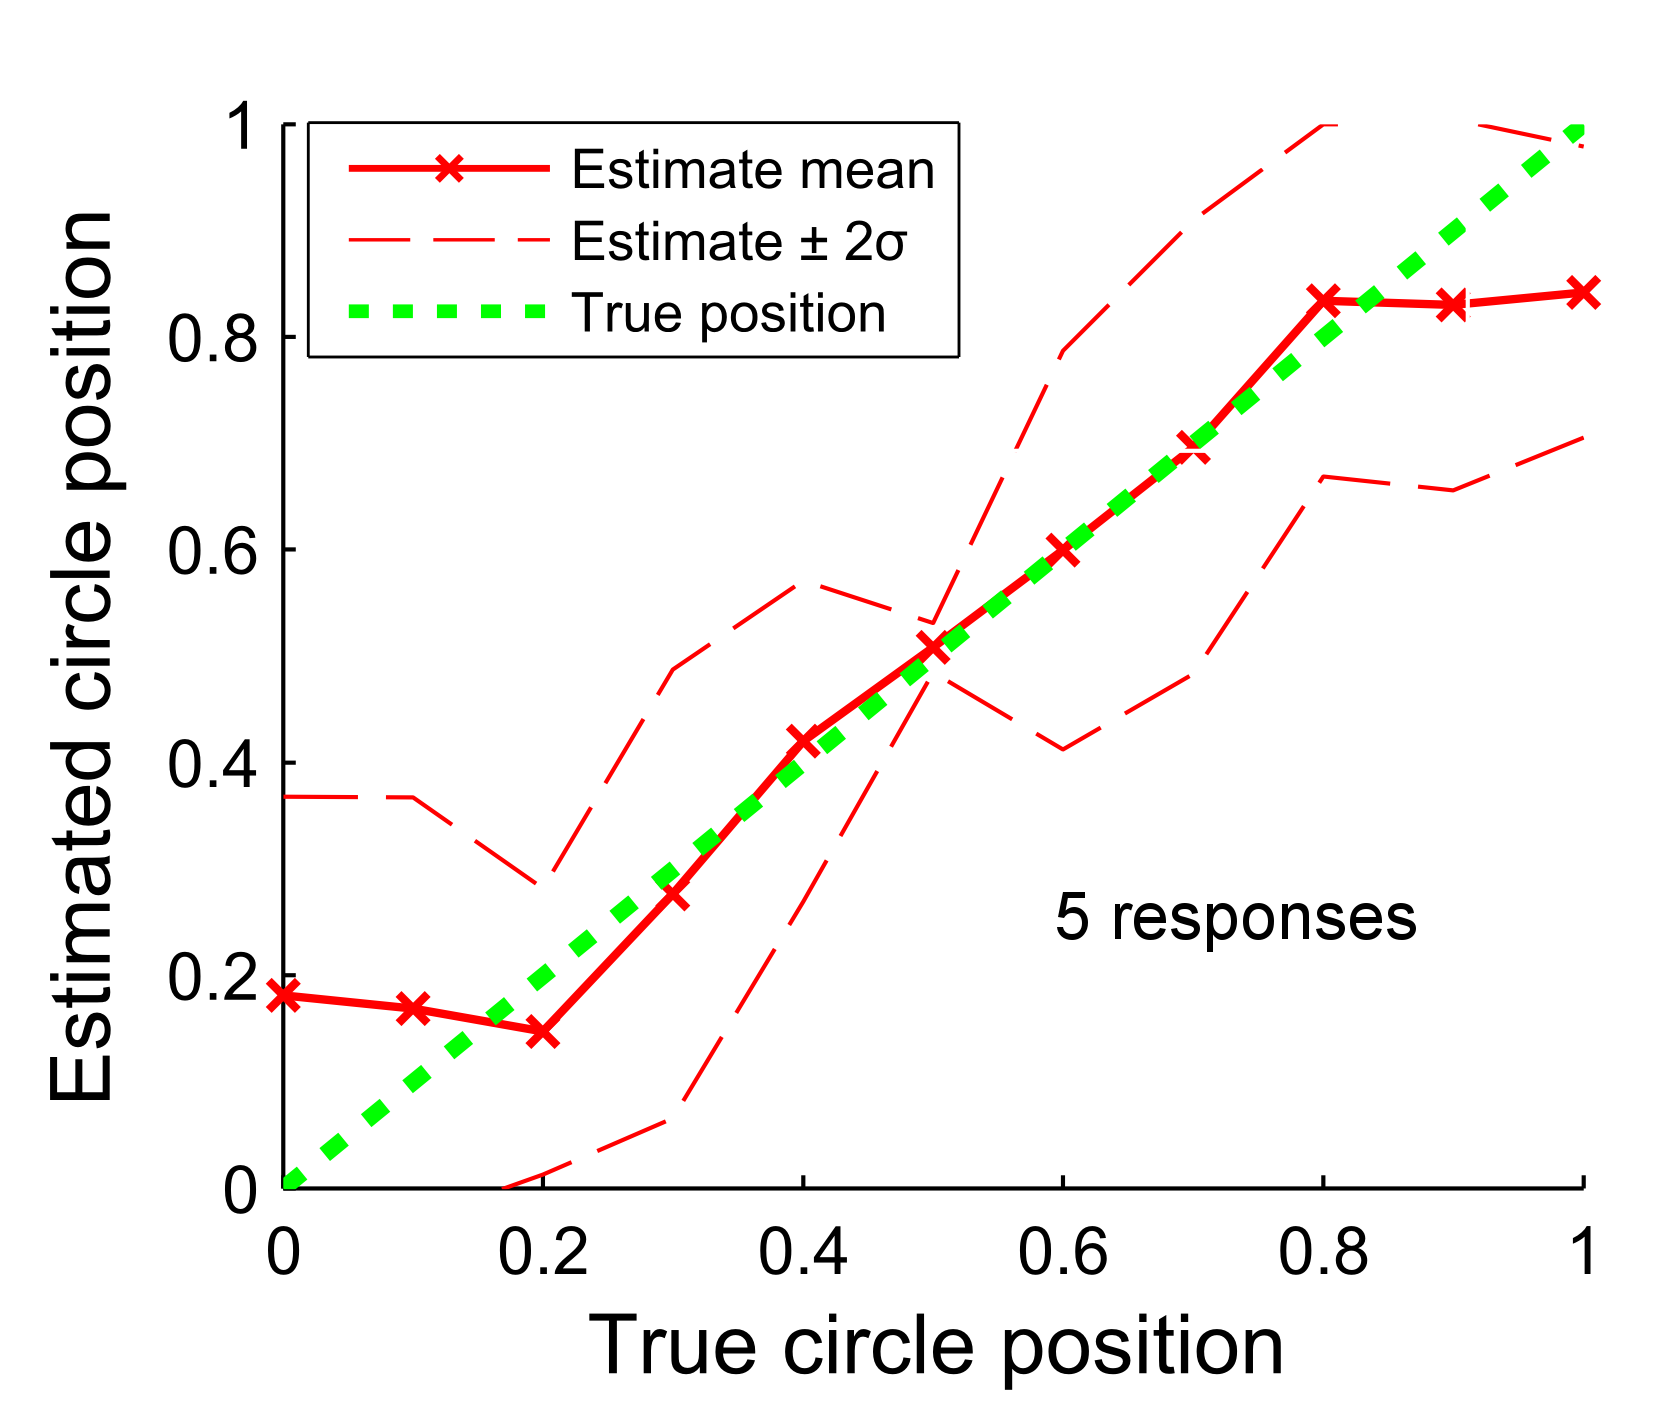
\includegraphics[width=6cm]{line_mc_5res_estimate.png}
\caption{}
\label{Figure: response_estimate_5}
\end{subfigure}\\
\begin{subfigure}{6cm}
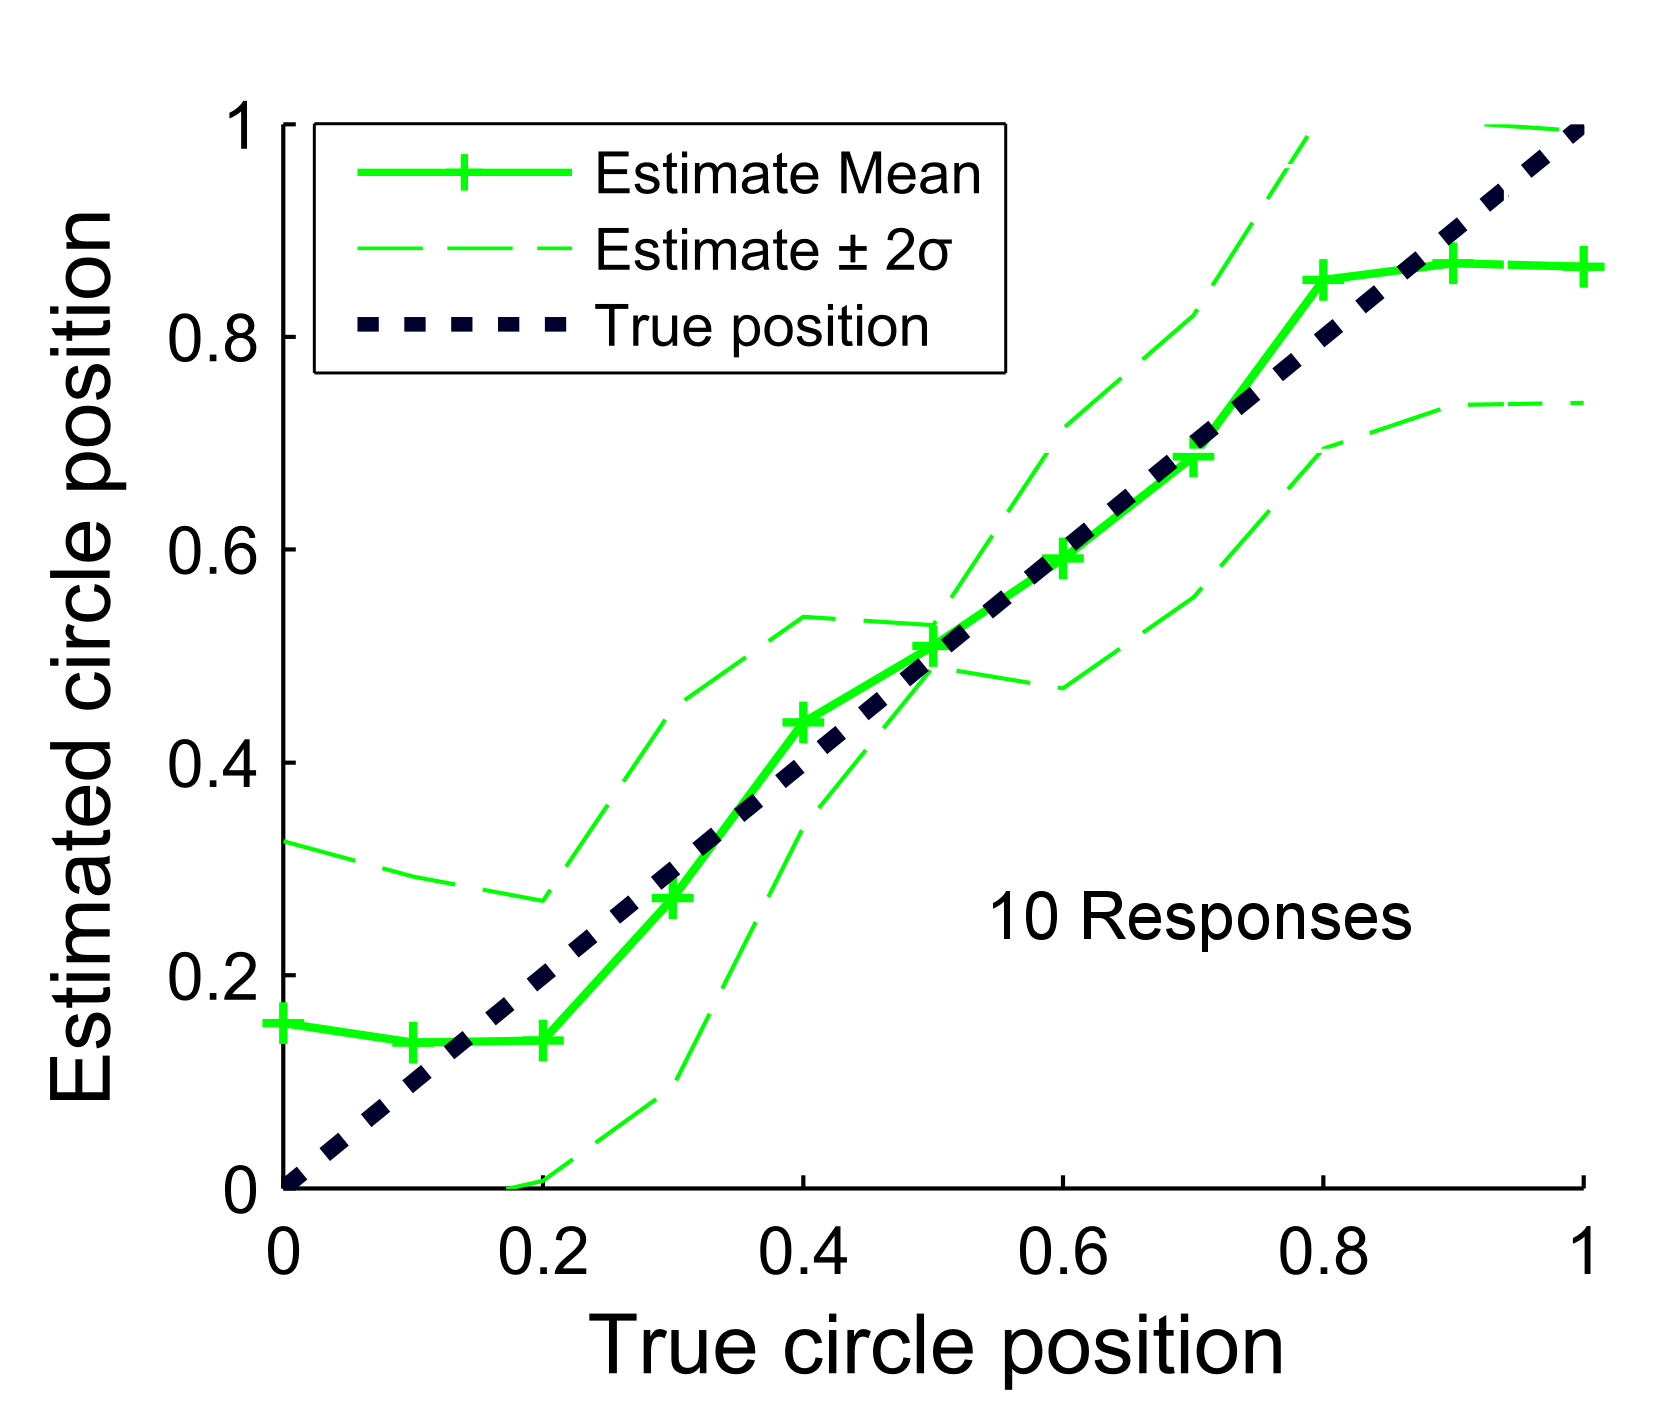
\includegraphics[width=6cm]{line_mc_10res_estimate.png}
\caption{}
\label{Figure: response_estimate_10}
\end{subfigure}
\begin{subfigure}{6cm}
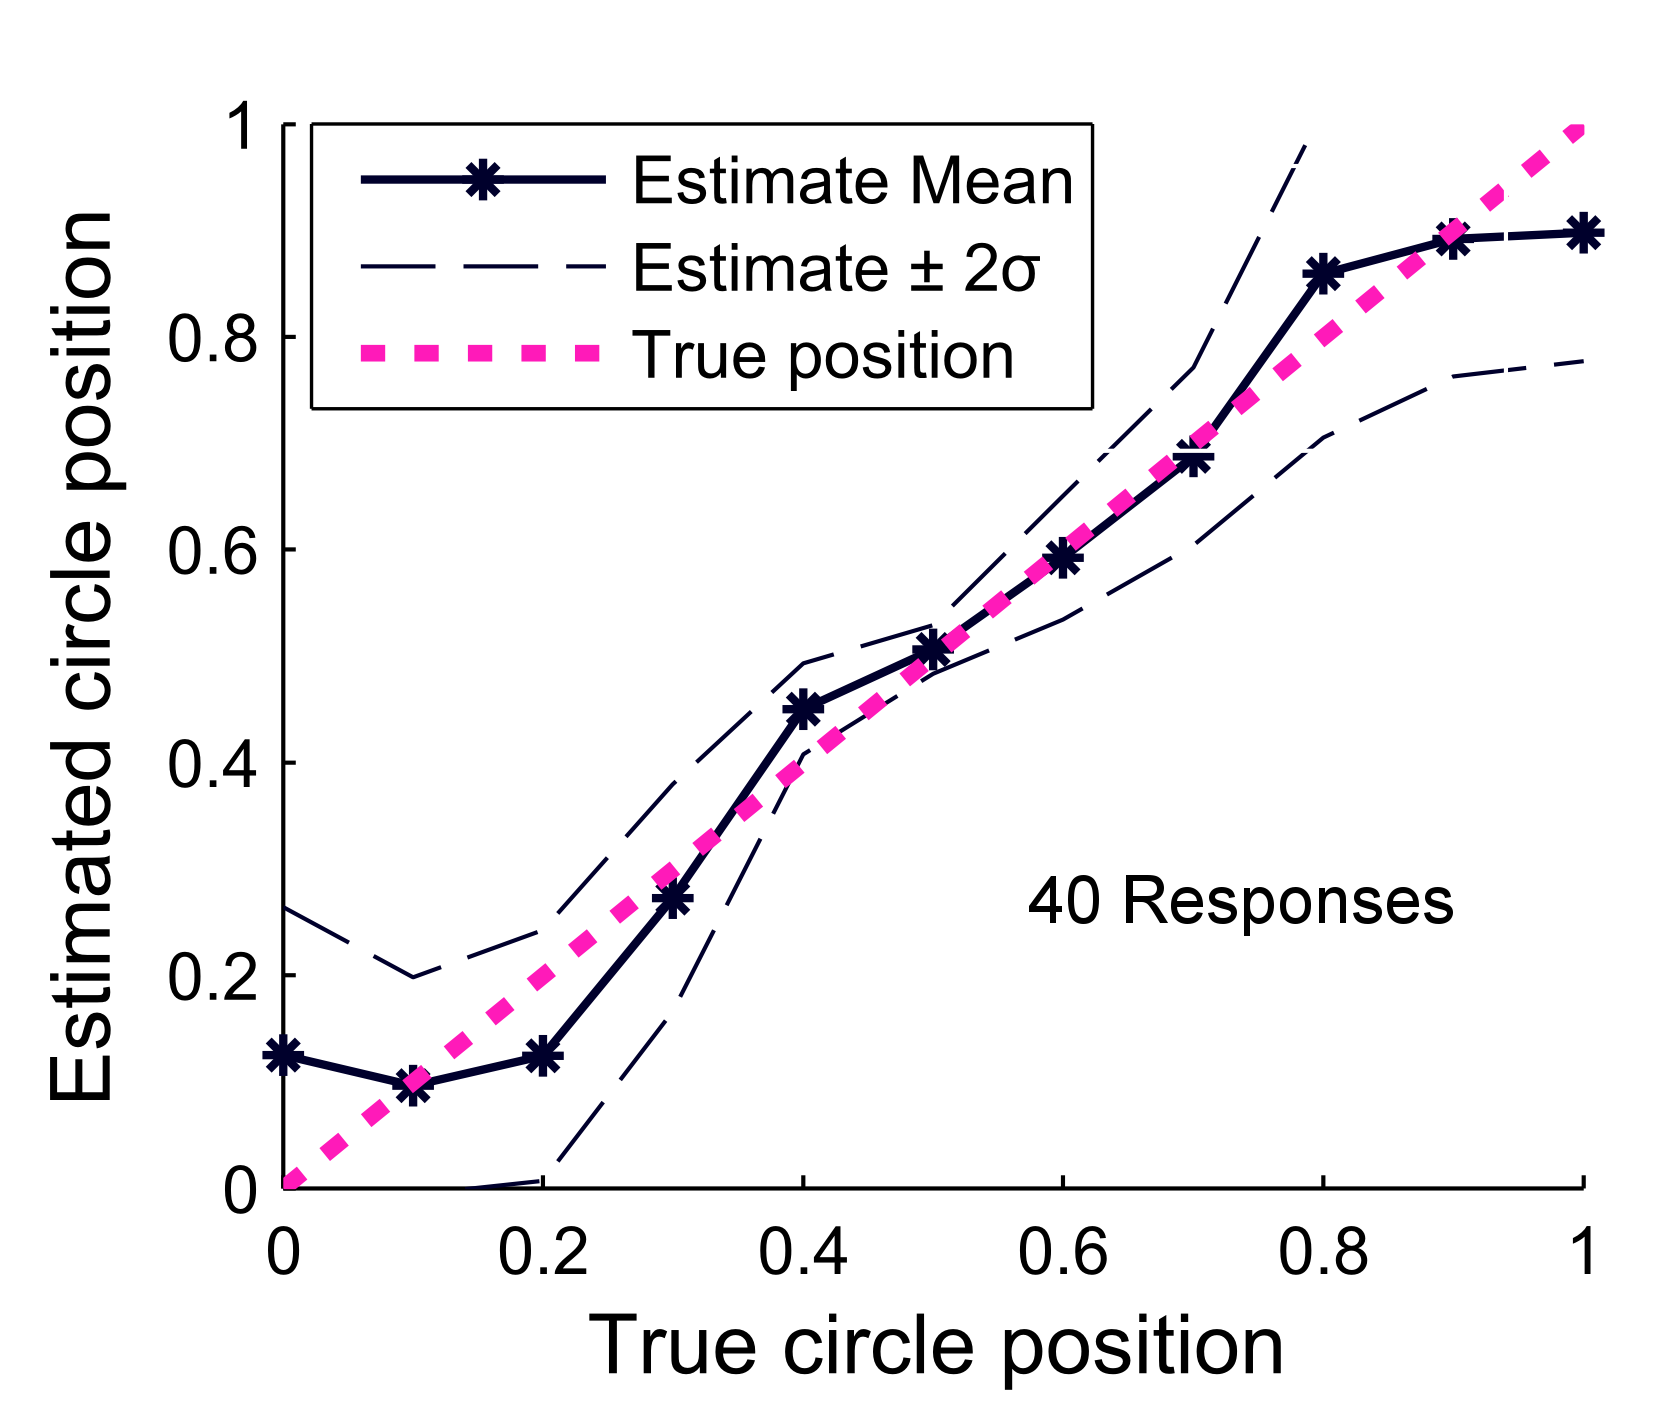
\includegraphics[width=6cm]{line_mc_40res_estimate.png}
\caption{}
\label{Figure: response_estimate_40}
\end{subfigure}
\caption{The mean performance of estimating the circle's position. The mean line is the average expectation value taken from 50 simulations runs. The standard deviations are for the deviations in the expectation values (not to be confused with the variance in the posterior distribution). The mean lines were generated using varying numbers of responses for each circle positon, with: \subref{Figure: response_estimate_1}) 1 response \subref{Figure: response_estimate_5}) 5 responses \subref{Figure: response_estimate_10})10 responses \subref{Figure: response_estimate_40}) 40 responses}
\label{Figure: response_estimate}
\end{figure}





\section{Limiting the worker variety/models}

It might seem intuitive to think that in an ideal world, for the purposes of data fusion, everyone would have the same response model i.e. the number of unique response models is one. That way we would know precisely the internal model that a person was using, and we could fit an accurate function to this. To test this intuition, a series of experiments were carried out in order to see the impact of limiting the variety of models found in the data. 

\subsection{Approach}

As shown in \ref{Figure:bar unique response model groups}, the number of unique models in the dataset with more than 1 worker associated to it was found to be 10. To investigate the impact of response model variety, these 10 models were used to create a series of training and testing datasets. 10 datasets were created in total.

The first dataset contained only the responses from the workers with the most popular response model, the model shown in \ref{Figure:one worker model}. This dataset contained the responses from 16 workers in total. The second dataset contained only the responses from the first and second most popular response models, which totalled 21 workers. This process was continued, with the tenth dataset containing the top 10 response models.

These datasets were then used to train the softmax model. As the datasets were now different sizes, only 8 randomly selected workers (half the number of workers in the first dataset) from each dataset were used to train the model, and then 8 remaining workers were randomly selected used to test the model. This process was carried out for 100 experimental runs for each dataset. 

\subsection{Model fitting}










\subsection{State Estimation Results}

\ref{Figure: fusion top 10 popular models} shows the results of fusing different numbers of models. In \ref{Subfigure:fusion 1-5 popular models}, we can see that using 1 response model, then our mean estimate of circle position after fusion essentially follows the response model - the shape is qualitatively the same.  As the number of models is increased, the mean estimate is improved. Increasing from 6-10 models shows little improvement in mean estimate. This is likely due to the small training and testing sets used. As response models 6-10 have relatively few workers in them compared to models 1-5, then the chances of them being sampled for training or testing purposes is relatively small.

%\begin{figure}
%	\centering
%		\begin{subfigure}{0.5\textwidth}
%			\centering
%			\setlength\figurewidth{10cm}
%    		\setlength\figureheight{10cm}  
%    		\inputTikZ{0.5}{line_models1-5_means.tikz}
%        	\subcaption{}\label{Subfigure:fusion 1-5 popular models}
%        \end{subfigure}%
%        \begin{subfigure}{0.5\textwidth}
%			\centering
%			\setlength\figurewidth{10cm}
%    		\setlength\figureheight{10cm}  
%    		\inputTikZ{0.5}{line_models6-10_means.tikz}
%    		\subcaption{}\label{Subfigure:fusion 6-10 popular models}
%        \end{subfigure}%
%        \caption{The mean estimate of circle position achieved by using 8 training workers and 8 testing workers over 100 simulation runs, sampled from datasets containing: \subref{Subfigure:fusion 1-5 popular models}) Top 5 popular response models; \subref{Subfigure:fusion 6-10 popular models}) Top 10 popular response models}
%        \label{Figure: fusion top 10 popular models}
%\end{figure}

In order to investigate the impact of the less popular response models, the same process was carried out using models 3-10. So for each dataset, the first two models were included. This increased the size of the dataset from 16, to 42 workers. The results are shown in \ref{Figure: fusion top 3-10 popular models}. These results show the same trend as the smaller dataset, with the increase in worker response models improving the data fusion results. The conclusion that can be drawn from this is that an increase in the variety of response models improves the overall fusion. We do not want all workers to behave the same, as is the case with 1 response model in \ref{Subfigure:fusion 1-5 popular models}. We want some spread of results, that gives each position of the circle as unique a input signature as possible. However, too much variety, and we would have an input that approximates noise.

%\begin{figure}
%	\centering
%		\begin{subfigure}{0.5\textwidth}
%			\centering
%			\setlength\figurewidth{10cm}
%    		\setlength\figureheight{10cm}  
%    		\inputTikZ{0.5}{line_models3-6_means.tikz}
%        	\subcaption{}\label{Subfigure:fusion 3-6 popular models}
%        \end{subfigure}%
%        \begin{subfigure}{0.5\textwidth}
%			\centering
%			\setlength\figurewidth{10cm}
%    		\setlength\figureheight{10cm}  
%    		\inputTikZ{0.5}{line_models7-10_means.tikz}
%    		\subcaption{}\label{Subfigure:fusion 7-10 popular models}
%        \end{subfigure}%
%        \caption{The mean estimate of circle position achieved by using 21 training workers and 21 testing workers over 100 simulation runs, sampled from datasets containing: \subref{Subfigure:fusion 3-6 popular models}) Top 6 popular response models; \subref{Subfigure:fusion 7-10 popular models}) Top 10 popular response models}
%        \label{Figure: fusion top 3-10 popular models}
%\end{figure}




%Figure, RMSE error for each number of models, with varaince in rmse over runs



%Variance should increase as the variety of dataset increases? 









\section{Data Filtering}

This section looks at the impact on the whole dataset using different data filtering approaches. 

\subsection{Common Models}

%FIGURE showing top 3, top 5, top 10



\subsection{Consistent Models}
%Figure showing all consistent,decreasing/increasing, and increasing only

\subsection{Symmetric Models}
%Figure showing all symmetric, and response symmetric


\subsubsection{}

\subsection{Gold Data Filtering}

\begin{figure}[!htb]
  \centering
  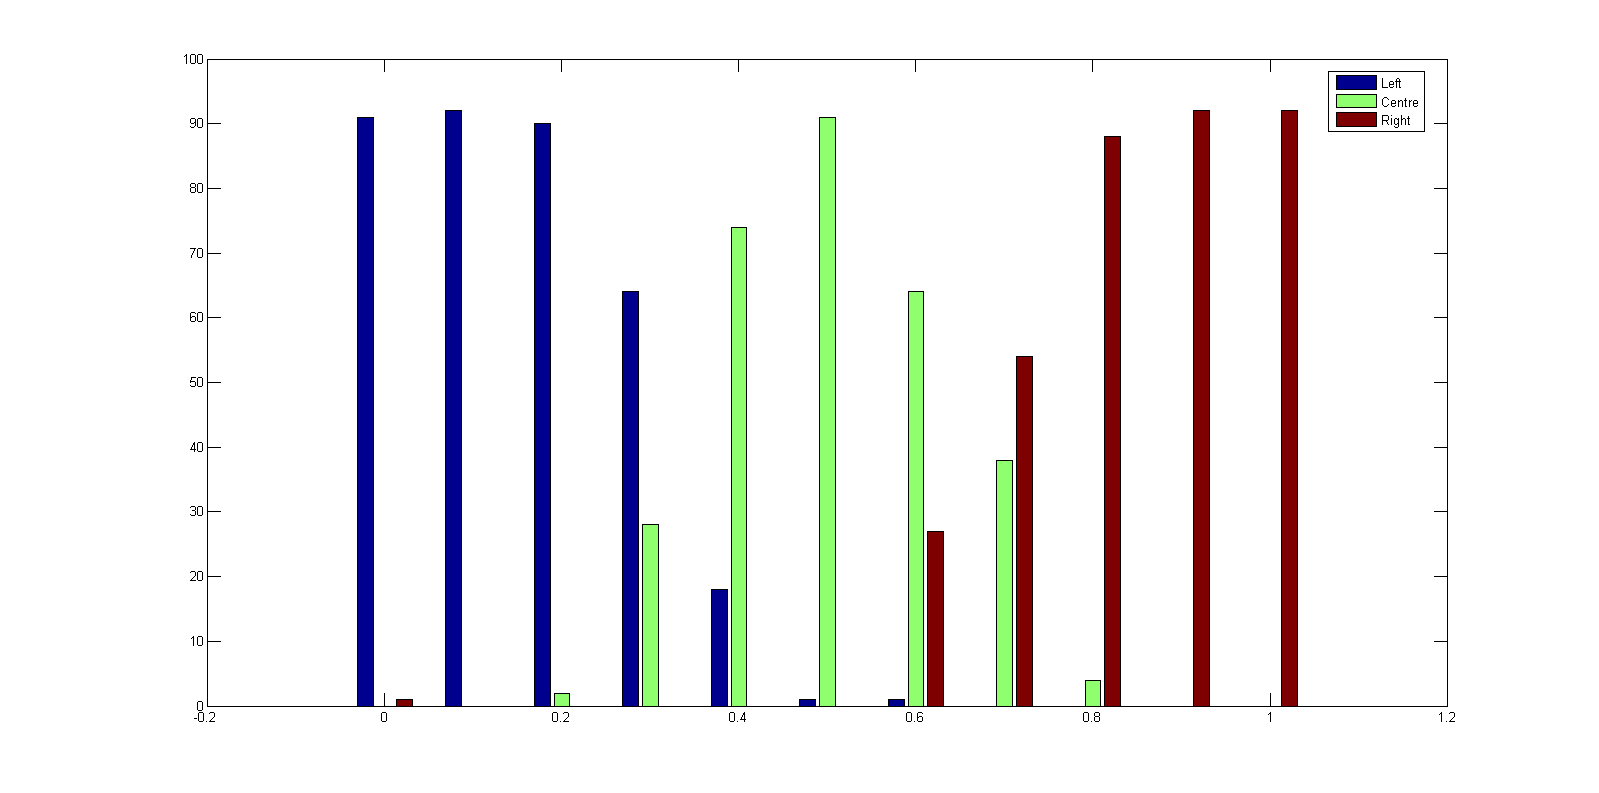
\includegraphics[width=8cm]{bar_responses_2_gold.png}
  \caption{The number of Left(Blue),Centre(Green) and Right(Red) worker responses at ground truth circle position after filtering the data using gold data and a threshold of 2 wrong answers}
  \label{Figure:bar responses 2 gold}
\end{figure}


%\begin{figure}[!htb]
%  \centering
%  \includegraphics[width=8cm]{bar_responses_1_gold.png}
%  \caption{The number of Left(Blue),Centre(Green) and Right(Red) worker responses at ground truth circle position after filtering the data using gold data and a threshold of 1 wrong answers}
%  \label{Figure:bar responses 1 gold}
%\end{figure}

Gold data filtering is a heuristic approach for filtering out poor performing workers. It relies on the creation of 'gold questions' ; questions where there is a known acceptable answer. In this experiment, there is ambiguity about where the classes NearToLeft, NearToCentre, and NearToRight start and finish. However, we would expect all responders to answer NearToLeft when the circle was located at 0, and NearToRight when the circle is located at 1. We can use these locations as gold questions, setting an expected response for each. If a worker gets a threshold value (or greater) of gold questions wrong, then we not only ignore their responses for the gold question, but also all other questions as they are deemed to be unreliable or of poor quality. 

Using the ground truth locations of 0 and 1 as gold questions, the data was filtered. Setting the threshold at 2 (workers who got both gold questions wrong were ignored), the filtered responses are shown in \ref{Figure:bar responses 2 gold}. 

Question IMPACT? Number of workers ignored? Worker responses? Graph them 

Question? Are all workers consistent? i.e. as x increases, once they switch from left to centre, do they stay at centre or do some go back to left???? 

The result of setting the gold data threshold to 1 is shown in \ref{Figure:bar responses 1 gold}. IMPACT - how many workers? What were that workers responses?

Total number of workers removed? Were any 'good' workers removed?


\subsection{Filtering comparisons}

%Table: Table showing the number of each report with each type of filtering, and the number of workers filtered out.